The simulator application is called rs for random schedule, lb for load balancer and sp for shortest path. To run the simulator, the following call may be executed:

\begin{figure}[h]
    \centering
    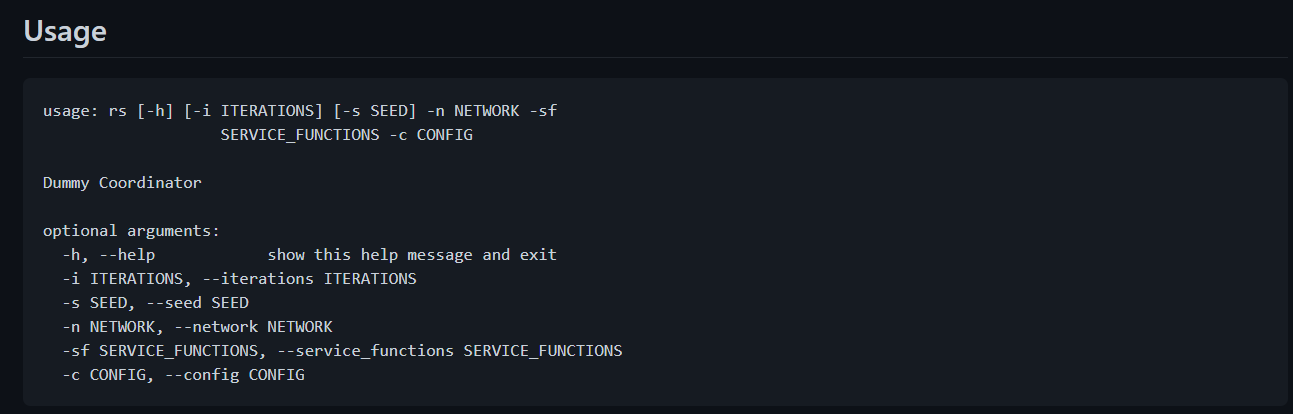
\includegraphics[width=1\textwidth]{terminal}
    \caption{commands usage}
    \label{fig:terminal}
\end{figure}

In our case we ran the following:

\begin{figure}[h]
    \centering
    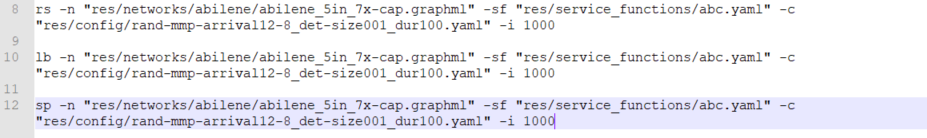
\includegraphics[width=1\textwidth]{commands}
    \caption{commands used in CLI}
    \label{fig:commands}
\end{figure}


And this is the output of the command running. ( LOG level set to INFO).

\begin{figure}[h]
    \centering
    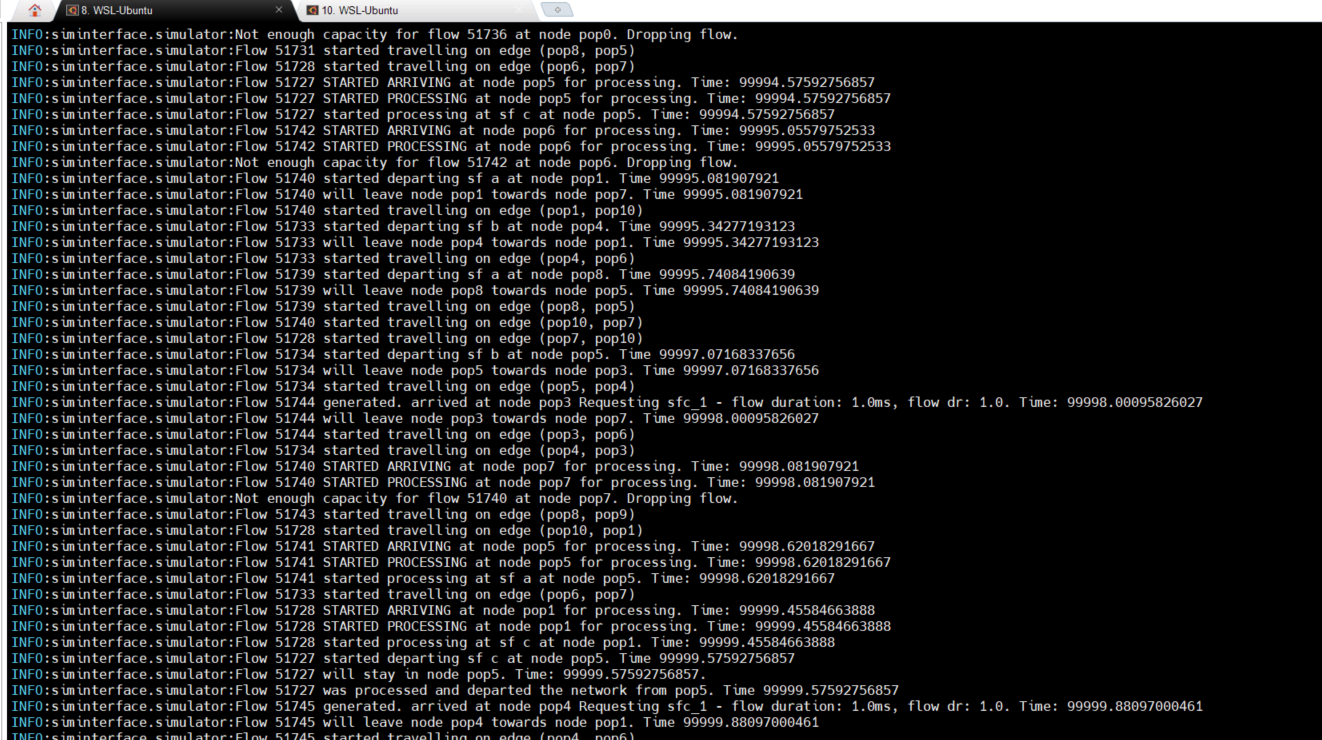
\includegraphics[width=1\textwidth]{simulation_info_level}
    \caption{commands running}
    \label{fig:simulation_info_level}
\end{figure}
